\documentclass[preprint,11pt,authoryear]{elsarticle}

\usepackage[T1]{fontenc}
\usepackage[utf8]{inputenc}
\usepackage{amsmath,amssymb}
\usepackage{booktabs,array}
\usepackage{graphicx}
\usepackage{xcolor}
\usepackage{tikz}
\usetikzlibrary{positioning,arrows.meta}
\usepackage[hidelinks]{hyperref}

\renewcommand{\bibfont}{\small}
\setlength{\bibsep}{1.5pt plus 0.5pt}
\graphicspath{{figures/}}
% Generated by scripts/paper_lic_rq_v2_assets.py
\newcommand{\nRecords}{11{,}382}
\newcommand{\nTasks}{48}
\newcommand{\nEmptyPrimaries}{6}
\newcommand{\nPermutations}{10{,}000}
\newcommand{\recordsSha}{e313f1ce5985}
\newcommand{\Ktemp}{0.7}
\newcommand{\Krep}{5}
\newcommand{\Lpar}{2}
\newcommand{\maxTok}{2{,}048}
\newcommand{\dialGpt}{0.688}
\newcommand{\freshGpt}{0.896}
\newcommand{\diffGpt}{0.208}
\newcommand{\ciGpt}{[0.063, 0.354]}
\newcommand{\pHolmGpt}{0.026}
\newcommand{\pRawGpt}{0.013}
\newcommand{\dialLlama}{0.854}
\newcommand{\freshLlama}{0.958}
\newcommand{\diffLlama}{0.104}
\newcommand{\ciLlama}{[0.000, 0.208]}
\newcommand{\pHolmLlama}{0.125}
\newcommand{\pRawLlama}{0.125}
\newcommand{\dialMistral}{0.063}
\newcommand{\freshMistral}{0.354}
\newcommand{\diffMistral}{0.292}
\newcommand{\ciMistral}{[0.146, 0.438]}
\newcommand{\pHolmMistral}{0.004}
\newcommand{\pRawMistral}{0.001}
\newcommand{\nFreshOnly}{34}
\newcommand{\nDialOnly}{5}
\newcommand{\crlAuroc}{0.627}
\newcommand{\crlCi}{[0.493, 0.760]}
\newcommand{\crlP}{0.022}
\newcommand{\crlPairs}{687}
\newcommand{\robAllAuroc}{0.571}
\newcommand{\robAllP}{0.057}
\newcommand{\robAllCi}{[0.484, 0.656]}
\newcommand{\robExclAuroc}{0.569}
\newcommand{\robExclP}{0.059}
\newcommand{\robExclCi}{[0.483, 0.655]}
\newcommand{\replayCandidates}{0}
\newcommand{\replaySensCandidates}{0}

% Generated by scripts/paper_merged_cdr_assets.py
\newcommand{\cdrSzeroEDialRange}{0.10--0.14}
\newcommand{\cdrSzeroECtrlRange}{0.82--0.86}
\newcommand{\cdrGptEarly}{0.61}
\newcommand{\cdrGptLate}{0.09}
\newcommand{\cdrGptCtrlLate}{0.64}
\newcommand{\cdrLlamaControlGap}{0.545}
\newcommand{\cdrLlamaControlCiLo}{0.513}
\newcommand{\cdrLlamaControlCiHi}{0.576}
\newcommand{\cdrLlamaControlHolmP}{$<$0.001}
\newcommand{\cdrLlamaControlLateGap}{0.575}
\newcommand{\cdrGemmaControlGap}{0.588}
\newcommand{\cdrGemmaControlCiLo}{0.557}
\newcommand{\cdrGemmaControlCiHi}{0.619}
\newcommand{\cdrGemmaControlHolmP}{$<$0.001}
\newcommand{\cdrGemmaControlLateGap}{0.630}
\newcommand{\cdrLevelMatched}{-0.118}
\newcommand{\cdrLevelMatchedP}{$<$0.001}
\newcommand{\cdrLevelMatchedN}{90}
\newcommand{\cdrLevelMatchedSzeroE}{-0.185}
\newcommand{\ctrlScreenDetect}{0/18}
\newcommand{\earlyCqSignal}{18/18}
\newcommand{\earlyCqNull}{3/12}
\newcommand{\earlyLsSignal}{10/18}
\newcommand{\earlyLsNull}{4/12}
\newcommand{\earlyLsBefore}{7}
\newcommand{\valLlamaDetect}{6/18}
\newcommand{\valLlamaDelay}{29}
\newcommand{\valLlamaLsSignal}{11/18}
\newcommand{\valLlamaLsNull}{6/12}
\newcommand{\valLlamaAggDetect}{3/3}
\newcommand{\valLlamaAggNull}{0/2}
\newcommand{\valGemmaDetect}{1/18}
\newcommand{\valGemmaDelay}{25}
\newcommand{\valGemmaLsSignal}{16/18}
\newcommand{\valGemmaLsNull}{3/12}
\newcommand{\valGemmaAggDetect}{3/3}
\newcommand{\valGemmaAggNull}{1/2}
\newcommand{\replaySsDeltaGpt}{+0.46}
\newcommand{\replaySsDeltaLlama}{+0.42}
\newcommand{\replayLsDeltaGpt}{+0.31}
\newcommand{\silentCQEarly}{0.61}
\newcommand{\silentCQLate}{0.08}
\newcommand{\silentCSEarly}{0.79}
\newcommand{\silentCSLate}{0.64}
\newcommand{\silentLSEarly}{0.54}
\newcommand{\silentLSLate}{0.47}
\newcommand{\silentSSEarly}{0.94}
\newcommand{\silentSSLate}{0.98}
\newcommand{\silentCsSupport}{2976}
\newcommand{\silentRsSupport}{427}
\newcommand{\crlLastGapAuroc}{0.672}
\newcommand{\crlLastGapP}{0.001}
\newcommand{\crlCondAuroc}{0.468}
\newcommand{\crlCondP}{0.674}


\makeatletter
\newcommand{\inputtable}[1]{\@@input #1 }
\makeatother

\newdefinition{definition}{Definition}
\newtheorem{proposition}{Proposition}
\newproof{pf}{Proof}

\journal{Information Sciences}

\begin{document}

\begin{frontmatter}

\title{The Silent Cost of Conversation History in LLM Reasoning}

\author[tarsus]{Ali \c{S}enol\corref{cor1}}
\ead{alisenol@tarsus.edu.tr}
\cortext[cor1]{Corresponding author.}
\affiliation[tarsus]{organization={Department of Computer Engineering, Tarsus University},
  city={Tarsus, Mersin}, postcode={33400}, country={T\"urkiye}}

\begin{abstract}
Large language models (LLMs) in multi-turn information systems keep their own
earlier replies and a growing task state in context. We asked whether this
conversation history lowers accuracy, and whether process-level quality
metrics warn before it does. Each analysis was fixed before its outcomes were
computed. In Study~1, on 48 sharded math tasks, retaining the model's replies
lowered final success by 0.21 for GPT-4o-mini and 0.29 for Mistral-7B
(Holm-adjusted $p=0.026$ and $0.004$); Llama-4 Scout moved in the same
direction without significance. Study~2 introduces CDR-Stream, 100-turn
state-tracking dialogues with an exact answer at every turn and difficulty
calibrated per model. With the full history, accuracy fell from about 0.6 to
0.1 within twenty turns at matched difficulty, whereas a solver-verified state
summary kept it 0.52--0.59 higher (Holm-adjusted $p<0.001$). Consistency and
logical coherence fell far less than accuracy, and stability rose. None
of these metrics, a paired readiness measure or calibrated single-stream drift
detectors gave robust, model-general early warning, although in Study~2 the
repeat-based metrics were complete only for GPT-4o-mini. In the monitors we
tested, a single 100-turn stream had power only for very large drops. Systems
built on LLMs should keep task state outside the transcript and monitor across
sessions.

\end{abstract}

\begin{keyword}
large language models \sep multi-turn dialogue \sep conversation history \sep
state tracking \sep reasoning quality \sep drift detection \sep early warning
\end{keyword}

\end{frontmatter}

\section{Introduction}
\label{sec:introduction}

LLMs are increasingly used as components of information and decision-support
systems that keep a task open over many turns. A procurement assistant tracks a
budget as invoices arrive; a logistics assistant follows stock across
warehouses. The user supplies information piece by piece and asks questions
whose answers depend on everything said so far, so the model's context fills
with its own earlier replies and with a task state that changes at every turn.
We call this accumulated context the \emph{conversation history}, and the
experimental condition that keeps it \emph{dialogue history}.

\paragraph{Why this is a reliability problem, not only an accuracy problem}
A growing conversation history can let a model lock onto a wrong task state:
once an early turn is answered incorrectly, every later reply can be generated
consistently from that wrong state, without the model producing any of the
usual symptoms of failure. If a deployed system does not see the gold answer,
and the responses it does see remain fluent, mutually consistent and locally
coherent, the failure is invisible unless some other signal flags it. The paper
asks two questions that follow from this chain: does retaining history cost
accuracy, and does that cost compound as the conversation grows; and if it
does, can the cost be seen before it shows up in the final answer, using
signals a deployed system can actually compute?

\paragraph{What is known}
Multi-turn use is known to be costly. Models lose accuracy when a task is
revealed over several turns because they commit to premature answers
\citep{laban2025lost}; earlier assistant replies can propagate errors
\citep{huang2026benefit}; and the effective context is shorter than the
nominal one \citep{liu2024lost,hsieh2024ruler}.

\paragraph{Two gaps these results leave open}
First, a \emph{measurement gap}: the cited studies score a single answer after
at most a handful of turns, so they show that history can hurt but not how the
loss develops over a long horizon. Over tens of turns, the questions themselves
may also become harder, so a falling accuracy curve can reflect the questions
rather than the context unless difficulty is explicitly held fixed. Second, a
\emph{monitoring gap}: none of these studies treats reasoning-quality metrics
as a stream, applies a detector calibrated on a stationary baseline, or reports
a false-alarm rate. Showing that performance eventually drops is not the same
as showing that the drop can be seen coming. ERGO is the closest exception, but
it monitors token-entropy spikes rather than response-level quality metrics,
and it is not evaluated against a long, difficulty-controlled horizon
\citep{khalid2025ergo}. To our knowledge, no prior study jointly (i) holds
difficulty fixed over a long multi-turn horizon and (ii) tests established
quality metrics as calibrated early-warning signals with a controlled
false-alarm rate.

\paragraph{This paper}
We close both gaps with two experiments, each analysed under a protocol fixed
before its outcomes were computed. Study~1 addresses the short-horizon
measurement gap directly: it compares, turn by turn, the same user information
with and without the model's own earlier replies. Study~2 addresses the
long-horizon and monitoring gaps together with CDR-Stream, a benchmark of
100-turn state-tracking dialogues with an exact answer at every turn,
difficulty calibrated per model, and a control arm that replaces the history
with a solver-verified state summary. The two studies differ in tasks, models
and controls, so we read them as two related failure modes rather than as one
dose--response curve.

The paper makes three contributions:
\begin{enumerate}
  \item a prospectively frozen, paired estimate of the cost of retaining
    assistant replies on short sharded tasks, which replicates the direction
    reported by \citet{huang2026benefit};
  \item CDR-Stream, a long-horizon, difficulty-calibrated benchmark in which
    accuracy under full history collapsed within about twenty turns at matched
    difficulty, while a verified state summary preserved it;
  \item a prospectively defined evaluation of whether established
    reasoning-quality metrics and calibrated single-stream detectors can
    serve as early warnings of this collapse -- assessing not only whether
    they move before accuracy fails, but whether any such lead survives a
    controlled false-alarm rate and repeats across models. None did: coherence
    and stability moved the wrong way, staying flat or rising as accuracy
    fell, and a closed-form bound together with a power simulation explains
    how much of this is a fundamental limit of single-conversation monitoring
    rather than a property of the metrics themselves.
\end{enumerate}

\section{Related work}
\label{sec:related}

\paragraph{Multi-turn and long-context degradation}
MT-Bench, MT-Eval and MINT evaluate conversational ability over several
exchanges \citep{zheng2023judging,kwan2024mteval,wang2024mint}.
\citet{laban2025lost} sharded fully specified tasks across turns and traced
large losses to premature answers on which models then anchored.
\citet{huang2026benefit} omitted or condensed assistant turns, including on the
Lost in Conversation math tasks, and found that earlier replies can propagate
errors, and \citet{sinha2025illusion} reported self-conditioning on earlier
errors in long-horizon execution. Related work documents information lost in
the middle of long inputs \citep{liu2024lost}, effective context below the
advertised length \citep{hsieh2024ruler}, distraction by irrelevant context
\citep{shi2023distracted}, sycophancy \citep{sharma2024sycophancy}, unreliable
self-correction \citep{huang2024cannot} and difficulty in tracking entity states
\citep{kim2023entity}. Memory architectures summarise or page earlier content
\citep{packer2023memgpt,zhong2024memorybank,wang2023recursive}, long-term
memory benchmarks test whether facts survive across sessions
\citep{maharana2024locomo,wu2025longmemeval}, and ERGO
rebuilds the prompt after spikes in token entropy \citep{khalid2025ergo}. Our
verified state summary is an upper reference for such compact memory, not a
deployable summariser.

This body of work documents four related but distinct phenomena: losing
information that sits in the middle of a long input, failing to keep a
changing task state consistent across turns, being misled by one's own
earlier (possibly wrong) replies, and being unable to tell, without the gold
answer, that any of the first three is happening. The first three describe
\emph{why} accuracy might fall; the fourth is the \emph{monitoring} question
this paper tests, and none of the studies above calibrates a detector against
it with a controlled false-alarm rate.

\paragraph{Reasoning quality and drift monitoring}
Reasoning quality has been characterised by agreement among sampled solutions
\citep{wang2023selfconsistency}, faithfulness of chains of thought
\citep{wei2022chain,turpin2023say,lanham2023measuring} and models' knowledge of
their own correctness \citep{kadavath2022know}; sample checks
\citep{manakul2023selfcheckgpt} and semantic entropy
\citep{farquhar2024detecting} estimate uncertainty without labels. Recent work
adapts clinical cognitive tests to LLMs \citep{park2027lmmse} and optimises the
steps of mathematical reasoning \citep{lee2026fgrpo}. These approaches judge one
response at a time; we instead ask whether the same signals, aggregated per
turn, anticipate a later failure. We use the six RQEval dimensions
\citep{rqeval2026} unchanged, rather than proposing new ones, because they
already span the two properties a label-free precursor would need: agreement
(CS, RS) across repeated or reworded answers, and internal coherence or
stability (LS, SS) of a single reasoning trace; CQ and ES require the gold
answer and serve only as the outcome being warned about. CUSUM
\citep{page1954continuous}, Page--Hinkley
\citep{hinkley1971inference}, EWMA \citep{roberts1959control}, DDM
\citep{gama2004learning} and ADWIN \citep{bifet2007learning} are standard
stream detectors whose delay and false alarms have been compared extensively
\citep{gama2014survey,webb2016characterizing,goncalves2014comparative,barros2018largescale,bayram2022concept};
recent methods classify drift types \citep{deng2025zilean} and couple
detection with adaptation \citep{abushaira2027sccm}. Such detectors usually
watch input distributions or labelled performance
\citep{sculley2015hidden,rabanser2019failing}, and commercial LLM behaviour is
known to drift \citep{chen2024chatgpt}. We apply them instead to per-turn
reasoning-quality streams within a conversation.

Table~\ref{tab:positioning} places our studies against the closest work. We do
not claim to be the first to show that assistant history can hurt; we add a
prospectively frozen paired estimate, exact per-turn answers over 100 turns at
calibrated difficulty, and a direct test of quality metrics and detectors as
early warnings.

\begin{table}[!htbp]
\centering
\caption{Positioning against the closest prior work.}
\label{tab:positioning}
\footnotesize
\setlength{\tabcolsep}{4pt}
\begin{tabular}{@{}>{\raggedright\arraybackslash}p{0.19\linewidth}
>{\raggedright\arraybackslash}p{0.25\linewidth}
>{\raggedright\arraybackslash}p{0.25\linewidth}
>{\raggedright\arraybackslash}p{0.25\linewidth}@{}}
\toprule
Study & Setting & Role of history & Signals for monitoring\\
\midrule
\citet{laban2025lost} & sharded single-turn tasks & cause of premature,
unreliable answers & not studied\\
\citet{huang2026benefit} & real and sharded conversations & assistant turns
omitted or condensed & not studied\\
\citet{sinha2025illusion} & synthetic long-horizon execution & self-conditioning
on own errors & not studied\\
ERGO \citep{khalid2025ergo} & sharded tasks & reset after uncertainty spikes &
token entropy as a trigger\\
Study 1 (ours) & sharded math tasks, paired arms & net effect of retaining
replies & CS, LS, SS and a paired readiness measure\\
Study 2 (ours) & 100-turn state tracking, calibrated difficulty & full history
versus verified state & six RQEval metrics, five detectors\\
\bottomrule
\end{tabular}
\end{table}

\section{Monitoring framework and evaluation design}
\label{sec:framework}

Both studies share the context policies, the per-turn quality signals, the
streaming monitor and the evidence standards defined here
(Figure~\ref{fig:framework}); Table~\ref{tab:datasets} summarises the two
benchmarks before the details below. Full model identifiers, gateway aliases
and acquisition dates are in supplementary Table~S18.

\begin{table}[!htbp]
\centering
\caption{The two benchmarks at a glance. K/L: same-context repeats / reworded
instructions per turn; ``full'' metric coverage means CQ, CS, RS, LS, ES and
SS, subject to the structural limits of Section~\ref{sec:framework} (CQ/RS/ES
need a final answer).}
\label{tab:datasets}
\footnotesize
\setlength{\tabcolsep}{4pt}
\begin{tabular}{@{}>{\raggedright\arraybackslash}p{0.17\linewidth}
>{\raggedright\arraybackslash}p{0.40\linewidth}
>{\raggedright\arraybackslash}p{0.40\linewidth}@{}}
\toprule
 & Study 1 (Lost in Conversation) & Study 2 (CDR-Stream)\\
\midrule
Source & GSM8K math, sharded \citep{cobbe2021training,laban2025lost} &
purpose-built, solver-checked\\
Units & \nTasks{} tasks, 4--9 turns (median 6) & 30 dialogues/model, 100 turns
each\\
Domains & arithmetic word problems & budget, inventory, lab, milestones (4)\\
Difficulty & not controlled & 12-level ladder, calibrated per model\\
Scenarios & single ordered reveal & 5 (2 stationary null, 3 scheduled-change)\\
Models & GPT-4o-mini, Llama-4 Scout, Mistral-7B & GPT-4o-mini, Llama-3 70B,
Gemma 3 12B\\
$K$ / $L$ & \Krep{} / \Lpar{}, all models & 3 / 2, GPT-4o-mini only\\
Metric coverage & full, pre-final turns only (no gold yet) & full for
GPT-4o-mini; CQ only for the other two\\
\bottomrule
\end{tabular}
\end{table}

\begin{figure}[!htbp]
\centering
\begin{tikzpicture}[
  font=\small, >=Latex, node distance=4mm and 6mm,
  box/.style={draw, rounded corners=2pt, align=center, minimum height=9mm,
              inner sep=3pt, fill=#1},
  box/.default=white]
\node[box=gray!10, text width=27mm] (user) {User turn $u_t$\\(new information,\\question)};
\node[box=blue!8, text width=33mm, right=of user] (policy)
  {Context policy $\pi$\\[1pt]\footnotesize dialogue history $\cdot$ fresh prefix\\
   \footnotesize $\cdot$ verified state summary};
\node[box=gray!10, text width=24mm, right=of policy] (llm) {LLM\\primary reply\\+ $K{-}1$ samples\\+ $L$ rewordings};
\node[box=orange!10, text width=26mm, below=9mm of llm] (metrics)
  {Per-turn quality\\vector $\mathbf{q}_t$\\\footnotesize CQ CS RS LS ES SS};
\node[box=orange!10, text width=27mm, left=of metrics] (window)
  {Window means\\$\bar q_{m,t}$ over the last\\$W$ valid values};
\node[box=red!8, text width=30mm, left=of window] (detect)
  {Drift detectors\\\footnotesize CUSUM, PH, EWMA,\\\footnotesize DDM, ADWIN};
\node[box=green!10, text width=30mm, below=8mm of detect] (alarm)
  {Alarm time $\tau_m$\\\footnotesize compared with the change $c$};
\node[box=green!10, text width=27mm, right=of alarm] (null)
  {Threshold from\\stationary nulls\\\footnotesize false alarms $\le\alpha$};
\node[box=gray!5, text width=26mm, right=of null] (gold)
  {Exact gold $y_t$\\\footnotesize(evaluation only)};
\draw[->] (user) -- (policy);
\draw[->] (policy) -- (llm);
\draw[->] (llm) -- (metrics);
\draw[->] (metrics) -- (window);
\draw[->] (window) -- (detect);
\draw[->] (detect) -- (alarm);
\draw[->, dashed] (null) -- (alarm);
\draw[->, dashed] (gold) -- (null);
\draw[->, dashed] (gold.north) -- (metrics.south);
\draw[->, dotted] (llm.north) -- ++(0,4mm) -| node[pos=0.25, above, font=\footnotesize]
  {primary reply enters later history (dialogue history only)} (policy.north);
\end{tikzpicture}
\caption{The monitoring framework. A context policy decides what the model
sees at turn $t$. Responses are scored into a per-turn quality vector, smoothed
over a window and passed to drift detectors whose thresholds are calibrated on
stationary dialogues. Exact gold is needed for CQ, RS and ES and for
evaluating alarms; CS, LS and SS do not use it.}
\label{fig:framework}
\end{figure}

\subsection{Context policies}

At turn $t$ the user sends $u_t$ and the model returns a primary reply $r_t$
from a context $C_t$ set by a policy $\pi$:
\begin{align}
  \text{dialogue history:}\quad & C_t = (u_1, r_1, \dots, r_{t-1}, u_t),\\
  \text{fresh prefix:}\quad & C_t = (u_1, \dots, u_t),\\
  \text{verified state summary:}\quad & C_t = (s_{t-1}, u_t),
\end{align}
where $s_{t-1}$ is the exact task state after turn $t-1$, rendered by a
solver. Dialogue history versus fresh prefix estimates the \emph{net} effect of
keeping assistant replies; context length and message positions also differ,
so the effect is not attributed to the content of the replies alone. The
verified state summary shortens the context, removes earlier replies and
supplies a correct state at once, so it tests a mitigation, not a mechanism.
Every context is packed into the request with server-side memory, retrieval and
prompt rewriting disabled, which makes it reproducible from the stored records.

\paragraph{A worked example (CDR-Stream)}
Suppose turn 7 reports ``warehouse~B received 40 crates of part~X,'' and turn
8 asks ``how many crates of part~X does warehouse~B hold now?'' Under
\emph{dialogue history}, $C_8$ is the full transcript of turns 1--8, including
whatever the model itself answered at every earlier turn; if an earlier update
or an earlier reply was wrong, $C_8$ still contains it, unflagged, alongside
the new turn. Under the \emph{verified state summary}, $C_8$ replaces that
transcript with the solver's current ledger for warehouse~B (one line per
part, with its correct running count) plus the new turn only; the model never
sees turns 1--7 or its own earlier replies. The gold answer is computed by the
same solver from the same ledger, independently of what either arm is shown.
Section~\ref{sec:study2} gives the full generator and prompt.

\subsection{Per-turn quality signals}

Each primary reply comes with $K-1$ further samples from the same context and
$L$ replies to frozen rewordings of the instruction. RQEval \citep{rqeval2026}
computes six dimensions in $[0,1]$, used unchanged: accuracy (CQ, the primary
answer equals the gold), consistency (CS, pairwise agreement of the $K$
answers), robustness (RS, agreement of reworded replies with a correct primary
answer), logical coherence (LS, absence of NLI contradictions between
consecutive steps; \citealp{he2021deberta}), efficiency (ES, correctness
combined with token economy) and stability (SS, BERTScore similarity of the $K$
traces; \citealp{zhang2020bertscore}). CQ, RS and ES need a final answer and the
gold, CS needs at least two answers, and LS and SS need only reasoning text.
Only LS and SS can therefore serve as label-free warnings before a model is
ready to answer. Concretely, LS splits a reply's reasoning into consecutive
steps, scores each adjacent pair for contradiction with an NLI model, and
reports one minus the mean contradiction probability, so a reply that never
contradicts itself scores 1 regardless of whether its conclusion is right. SS
instead compares the $K$ sampled \emph{replies} to the same context pairwise by
BERTScore and reports their mean similarity, so near-duplicate phrasing across
samples raises SS even when the shared answer is wrong. Both are computed only
when the reasoning text itself is present and parseable; missing values are
never imputed and are reported with their support (supplementary
Section~S1.2 gives the exact splitting and scoring rules).

\subsection{The streaming monitor}

Let $q_{m,t}\in[0,1]$ be the value of metric $m$ at turn $t$, or missing.

\begin{definition}[Window mean]
Let $V_{m,t}$ be the set of the last $W$ turns $j\le t$ at which $q_{m,j}$ is
observed. Once $|V_{m,t}|=W$, the monitored statistic is
\begin{equation}
  \bar q_{m,t} = \frac{1}{W}\sum_{j\in V_{m,t}} q_{m,j},
  \qquad W\in\{10,20,30\},
  \label{eq:windowmean}
\end{equation}
with $W=20$ primary. Missing values neither enter nor advance the window.
\end{definition}

Five detectors, CUSUM, Page--Hinkley, EWMA, DDM and ADWIN, are assigned to
metrics by three strategies fixed in the funded project design: CUSUM on every
metric, a distribution-specific mapping, and ADWIN on every metric
(supplementary Table~S8).

\begin{definition}[Alarm, calibration and detection]
For a detector with threshold $h$ reading $\bar q_{m,1},\dots,\bar q_{m,t}$,
the alarm time in a stream of $T$ turns is
\begin{equation}
  \tau_m(h) = \min\{t\le T : \text{the detector alarms at } t\},
  \label{eq:alarm}
\end{equation}
with $\tau_m=\infty$ if no alarm occurs. The threshold $h^\ast$ is the most
sensitive grid value whose first-alarm rate on stationary streams,
$\widehat{P}_0(\tau_m(h)\le T)$, is at most $\alpha$; drift data are never used.
For a change at turn $c$, an alarm is a \emph{false alarm} if
$\tau_m(h^\ast)<c$ and a \emph{detection} if $c\le\tau_m(h^\ast)\le c+33$.
\end{definition}

Study~1 estimates $\widehat{P}_0$ from permutation nulls with family-wise
$\alpha=0.05$, Study~2 from its stationary dialogues. Detecting a scheduled
change within 33 turns is not yet a warning. We call a signal an \emph{early
warning} only if, in addition, it alarms before the accuracy (CQ) alarm in the
same dialogue, keeps the null calibration, and does both across models.

\subsection{A paired readiness measure}

Sharded tasks allow an answer-free paired signal. Let $a_t^{\mathrm{F}}$ and
$a_t^{\mathrm{D}}$ be 1 if the fresh-prefix and dialogue-history arms attempt an
answer at turn $t$, and 0 if they ask for more information. The
\emph{Cumulative Resolution Lag} of a task is
\begin{equation}
  \mathrm{CRL} = \frac{1}{|\mathcal{T}|}\sum_{t\in\mathcal{T}}
  \max\!\left(a_t^{\mathrm{F}}-a_t^{\mathrm{D}},\,0\right),
\end{equation}
over the pre-final turns $\mathcal{T}$ at which both arms responded validly. It
measures how persistently the history arm lags an information-matched
counterfactual in becoming ready to answer, and it was fixed as an auxiliary
measure before the Study~1 data were collected.

\subsection{Evidence standards}

Each result carries one of four labels: \emph{confirmatory} (a hypothesis fixed
before its outcomes were computed), \emph{prespecified secondary},
\emph{exploratory} (rules fixed before computation on data already seen) or
\emph{post hoc}. In Study~1 the whole protocol, including the analysis, was
frozen before data collection. In Study~2 the design, sample, difficulty
mappings, prompt and truncation policy were frozen before the main run; the
analysis protocol was frozen when a budget pause had left 25,039 of 54,000
calls complete, before any main-run metric was computed (dated timeline in
supplementary Table~S19). Raw responses are stored before
scoring and never overwritten, failed gates are reported rather than
relabelled, and every number, table and figure is regenerated by scripts from
hashed inputs.

\section{Study 1: the paired effect of retaining assistant replies}
\label{sec:study1}

\subsection{Design}

\paragraph{Tasks and models}
We used the math subset of Lost in Conversation \citep{laban2025lost}: 103
GSM8K-derived problems \citep{cobbe2021training}, each split into ordered
information shards revealed one per turn. Before any model call, an input audit
excluded 17 tasks that duplicated our earlier inputs or appeared to change
meaning when sharded. A hash-based procedure that used no model output then
drew \nTasks{} tasks with 4--9 shards (median 6), plus four disjoint tasks used
only for technical integration. GPT-4o-mini \citep{openai2024gpt4o}, Llama-4
Scout and Mistral-7B \citep{jiang2023mistral} answered every turn in both arms
of Section~\ref{sec:framework}. Replies had to end with
\texttt{FINAL\_ANSWER: <number>} or \texttt{STATUS: NEED\_MORE\_INFORMATION}.
Each cell received $K=\Krep{}$ same-context samples and $L=\Lpar{}$ replies to
frozen instruction rewordings at temperature \Ktemp{}; only the primary entered
later history. All \nRecords{} calls succeeded without truncation. Six empty
Mistral-7B primaries were kept as invalid and transported by a fixed
placeholder. Prompts, the parser and the audit are detailed in the supplement.

\paragraph{Frozen analysis}
The primary endpoint was paired final-turn success, tested by exact McNemar
tests \citep{mcnemar1947note} with task-bootstrap 95\% CIs (\nPermutations{}
resamples; \citealp{efron1979bootstrap}) and Holm correction across models
\citep{holm1979simple}. Before the last shard most tasks have no determined
answer, so CQ, RS and ES are structurally unobservable there; the pre-final
warning candidates were CS, LS and SS. Each was tested by a task-clustered
partial correlation with final failure, adjusted for model, turn, revealed
information and log context length, with Holm correction across the three
metrics. CRL was frozen as an auxiliary measure; its target was a positive
final readiness gap, in which the fresh prefix attempts an answer while the
history arm remains unresolved.

\subsection{Results}

\paragraph{Retaining assistant replies lowers final success (confirmatory)}
Final success fell from \freshGpt{} to \dialGpt{} for GPT-4o-mini (difference
\diffGpt{}, 95\% CI \ciGpt{}, Holm $p=\pHolmGpt$) and from \freshMistral{} to
\dialMistral{} for Mistral-7B (\diffMistral{}, CI \ciMistral{}, Holm
$p=\pHolmMistral$); Llama-4 Scout showed the same direction (\diffLlama{}, CI
\ciLlama{}, Holm $p=\pHolmLlama$) without significance
(Table~\ref{tab:s1primary}, Figure~\ref{fig:s1}). Summed over models, only the
fresh prefix succeeded in \nFreshOnly{} model--task pairs and only the history
arm in \nDialOnly{}. A format-valid sensitivity analysis left the GPT-4o-mini
and Mistral-7B effects intact (supplementary Table~S1).
Mistral-7B illustrates one route to the harm: with its own replies in context
it tended to remain in an explicit ``need more information'' state at the last
turn, whereas without them it attempted an answer.

\begin{table}[!htbp]
\centering
\caption{Study 1 paired final-turn success over \nTasks{} tasks per model.
F/D: tasks in which only the fresh prefix, or only the dialogue history,
succeeded; $p$: exact McNemar test.}
\label{tab:s1primary}
\small
\resizebox{\linewidth}{!}{%
\begin{tabular}{lcccccc}
\toprule
Model & Dialogue history & Fresh prefix & Diff.\ [95\% CI] & F/D & $p$ & $p_{\text{Holm}}$\\
\midrule
\inputtable{generated/table_primary.tex}
\bottomrule
\end{tabular}
}
\end{table}

\begin{figure}[!htbp]
\centering
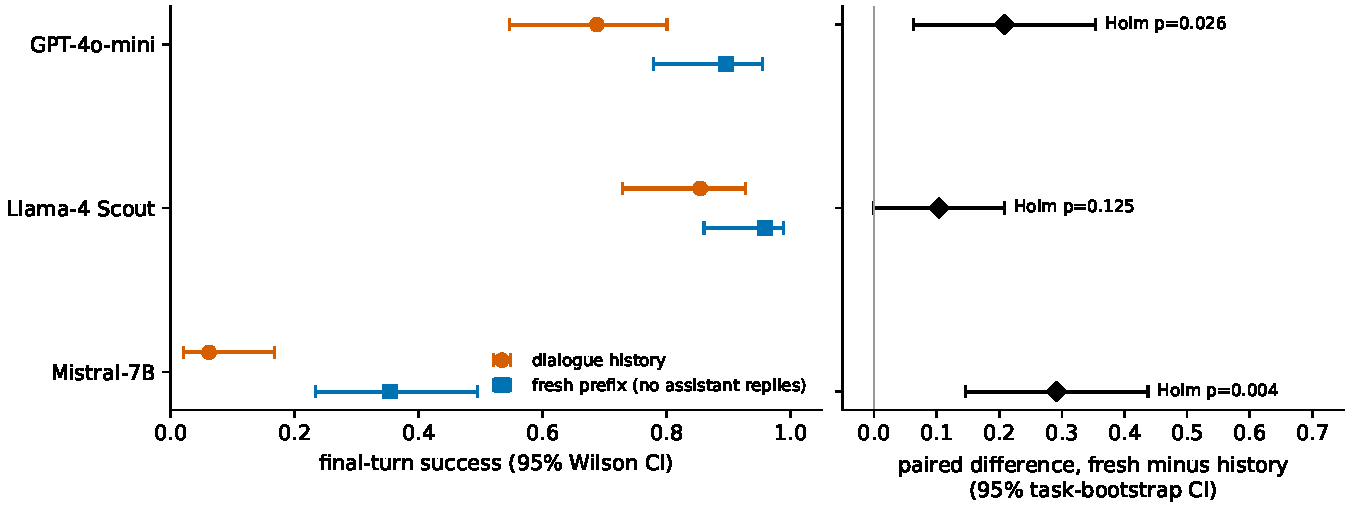
\includegraphics[width=\linewidth]{study1_paired.pdf}
\caption{Study 1 primary endpoint ($n=\nTasks{}$ paired tasks per model).
Left: final-turn success with 95\% Wilson intervals \citep{wilson1927probable}.
Right: paired difference, fresh prefix minus dialogue history, with 95\%
task-bootstrap intervals and Holm-adjusted McNemar $p$-values.}
\label{fig:s1}
\end{figure}

\paragraph{The measurable quality metrics do not warn (confirmatory)}
Under this analysis, CS, LS and SS showed no statistically detectable
association with final failure beyond turn, revealed information and context
length: all partial correlations were close to zero and every Holm-adjusted
$p$-value was 1.0 (Table~\ref{tab:s1rqeval}). This does not show that the
metrics carry no information. CS in particular was measurable on only 29 source
tasks, so small associations cannot be excluded.

\begin{table}[!htbp]
\centering
\caption{Study 1 pre-final metrics as predictors of final failure under
dialogue history ($r_{\text{partial}}$: task-clustered partial correlation;
$p$: one-sided task-clustered permutation test).}
\label{tab:s1rqeval}
\small
\begin{tabular}{lcccccc}
\toprule
Metric & Turns & Units & Tasks & $r_{\text{partial}}$ & $p$ & $p_{\text{Holm}}$\\
\midrule
\inputtable{generated/table_rqeval.tex}
\bottomrule
\end{tabular}
\end{table}

\paragraph{The paired readiness measure reduces to persistence}
CRL discriminated its frozen target modestly (pooled model-stratified AUROC
\crlAuroc{}, permutation $p=\crlP$, CI \crlCi{}; per-model results in
supplementary Table~S2). Post hoc, however, the last pre-final
readiness gap alone did better (AUROC \crlLastGapAuroc{}, $p=\crlLastGapP$),
and within its strata CRL added nothing (AUROC \crlCondAuroc{}, $p=\crlCondP$).
Against accuracy loss as a post-hoc target the association was borderline
(AUROC \robAllAuroc{}, $p=\robAllP$) and came from Mistral-7B alone. Even a
paired, counterfactual measure therefore registered the failure once the
history arm had fallen behind, rather than anticipating it.

\section{Study 2: long-horizon degradation under calibrated difficulty}
\label{sec:study2}

Study~1 tasks span at most nine turns, and their difficulty is not controlled.
In long dialogues the questions themselves may become harder, so a falling
accuracy curve could reflect the questions rather than the context. Study~2
therefore uses a purpose-built benchmark with an exact answer at every turn and
difficulty set by design.

\subsection{The CDR-Stream benchmark and design}

\paragraph{Dialogues}
CDR-Stream contains 100-turn dialogues in four state-tracking domains: a budget
ledger, inventory across warehouses, a laboratory protocol with container
volumes, and chains of project milestones. Each user turn states events that
update a shared state, such as a delivery, a transfer or a correction, possibly
with distractor sentences, and asks one question: a sum, a difference, a count
above a threshold, a maximum, a what-if or a share. An exact solver computes
the gold answer of every turn.

\paragraph{Calibrated difficulty and scenarios}
Difficulty follows a 12-level ladder that changes one axis per step: query
terms, events per turn, distractors or event complexity (supplementary
Table~S4). Before any stream existed, a single-turn calibration
mapped easy, medium and hard regimes to ladder levels for each model and domain,
targeting accuracy bands of 0.75--0.92, 0.60--0.78 and 0.35--0.65, and a frozen
rule (isotonic fit, \citealp{barlow1972statistical}; one-sided Cochran--Armitage
trend test, \citealp{armitage1955tests}; minimum regime gaps) excluded domains
with a ceiling, a floor or no trend (supplementary Table~S5). Each
model is thus evaluated in its own informative range, at the cost of models not
all being tested on the same set of domains; CDR-Stream is not designed to
rank models against each other, and we do not compare raw accuracy across
models for this reason. Five scenarios fix the
regime sequence: stationary easy (S0-E) and hard (S0-H), which serve as
monitoring nulls; a staircase from easy to hard with changes at turns 34 and 68
(S1); a sudden easy-to-hard shift at turn 51 (S2); and easy to hard to easy
with changes at 34 and 67 (S3); within a regime, levels are mixed around the
centre level (supplementary Section~S2.2).

\paragraph{Models, arms and analysis}
GPT-4o-mini, Llama-3 70B \citep{grattafiori2024llama3} and Gemma 3 12B
\citep{gemma2025gemma3} were retained because they passed calibration and a
technical pilot, before any stream outcome existed; replaced candidates and two
disclosed deviations for Llama-3 70B are documented in the supplement. Each
model received 30 held-out dialogues, six per scenario, in two arms: dialogue
history, and the verified state summary with the current turn. Both arms used
the same prompt and contract (at most eight numbered reasoning lines followed by
\texttt{FINAL\_ANSWER: <integer>}), temperature 0.7 and a 2,048-token ceiling.
The dialogue arm also drew $K=3$ samples and $L=2$ rewordings per turn;
because the research budget staged acquisition, these were completed only for
GPT-4o-mini. Truncated replies were kept and scored as missing under a policy
frozen before the main run. Dialogues are the independent units. A
prespecified secondary contrast compares accuracy at turns 1--50 and 51--100 at
the same ladder level within each dialogue -- holding question-side difficulty
fixed (query terms, events per turn, distractors and event complexity), not
the conversation length or the accumulated state, since those grow across
turns under both arms by design. The confirmatory hypothesis H-C1 states that,
for Llama-3 70B and Gemma 3 12B, per-dialogue accuracy over turns 1--100 is
higher under the verified state summary, tested by one-sided sign-flip tests
over 30 dialogues (20,000 draws;
\citealp{good2005permutation}) with bootstrap intervals and Holm correction.
GPT-4o-mini control data had been seen before this protocol and are reported
outside the family.

\subsection{Results}

\paragraph{Accuracy collapses under accumulated history}
In all three models, dialogue-history accuracy fell from about 0.6 in the first
five turns to about 0.1 after turn 20 (Table~\ref{tab:s2collapse},
Figure~\ref{fig:s2}a). The curves of the three models were nearly identical
despite different sizes and mappings, and the collapse appeared in every
scenario. In stationary easy dialogues, where the questions never became
harder, accuracy over turns 21--100 was \cdrSzeroEDialRange{} under dialogue
history against \cdrSzeroECtrlRange{} under the verified state summary. At the
same ladder level, late turns were less accurate than early turns by
\cdrLevelMatched{} (prespecified secondary, $p$~\cdrLevelMatchedP{},
$n=\cdrLevelMatchedN$ dialogues; \cdrLevelMatchedSzeroE{} in S0-E). Because most
of the decline occurs in the first half, this contrast understates the total
loss. The collapse also hides the scheduled task drifts: it is present in
stationary dialogues and begins before any detector could form a baseline, so
pre/post contrasts around the scheduled changes mix the two (supplementary
Table~S7).

\begin{table}[!htbp]
\centering
\caption{Study 2 accuracy (CQ) by turn range under dialogue history, pooled and
in the stationary easy scenario (S0-E), and under the verified state summary
(turns 21--100). Thirty dialogues per model.}
\label{tab:s2collapse}
\small
\begin{tabular}{lccccc}
\toprule
 & \multicolumn{3}{c}{Dialogue history, turns} & S0-E, & State summary,\\
\cmidrule(lr){2-4}
Model & 1--5 & 6--20 & 21--100 & turns 21--100 & turns 21--100\\
\midrule
\inputtable{generated/table_cdr_collapse.tex}
\bottomrule
\end{tabular}
\end{table}

\begin{figure}[!htbp]
\centering
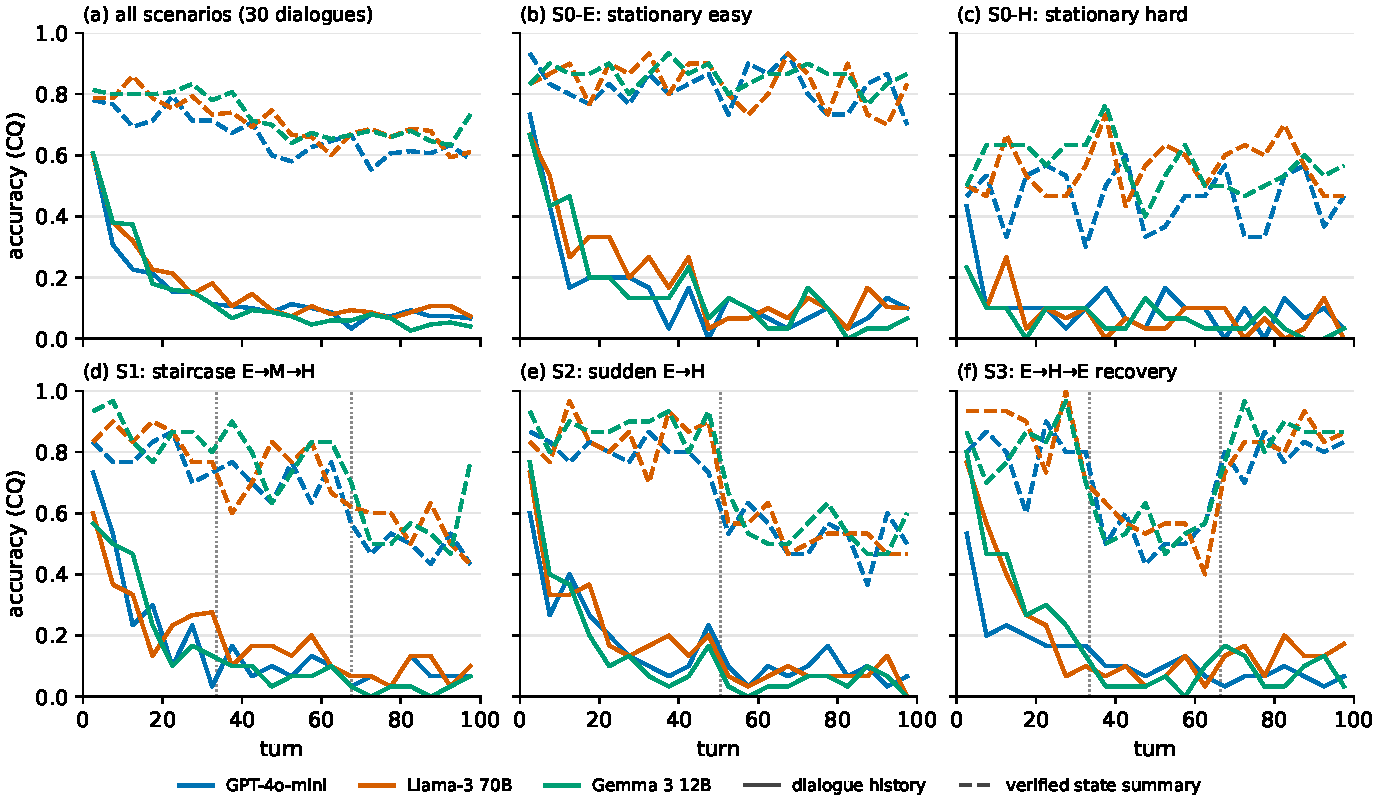
\includegraphics[width=\linewidth]{study2_accuracy_over_turns.pdf}
\caption{Study 2 accuracy over 100 turns in 5-turn bins: (a) all 30 dialogues
per model; (b)--(f) the five scenarios, six dialogues per model each. Solid:
dialogue history; dashed: verified state summary; dotted vertical lines:
scheduled difficulty changes.}
\label{fig:s2}
\end{figure}

\paragraph{A verified state summary preserves accuracy (confirmatory)}
Under the verified state summary, accuracy stayed high and followed the
difficulty schedule, stepping down at the changes of S1 and S2 and recovering in
the final easy regime of S3, a recovery that dialogue history never showed
(Figure~\ref{fig:s2}). H-C1 was supported for both members of the family
(Table~\ref{tab:s2control}): over turns 1--100 the gap was
\cdrLlamaControlGap{} for Llama-3 70B and \cdrGemmaControlGap{} for Gemma 3 12B
(Holm $p$~\cdrLlamaControlHolmP{} and \cdrGemmaControlHolmP{}), and over turns
21--100 it was \cdrLlamaControlLateGap{} and \cdrGemmaControlLateGap{}.
GPT-4o-mini showed the same direction.

\begin{table}[!htbp]
\centering
\caption{Frozen test H-C1: per-dialogue accuracy of the verified state summary
minus dialogue history over turns 1--100. GPT-4o-mini was observed before the
protocol and is outside the Holm family.}
\label{tab:s2control}
\small
\begin{tabular}{lcccc}
\toprule
Model & Mean gap & 95\% bootstrap CI & Holm $p$ & Dialogues\\
\midrule
\inputtable{generated/table_cdr_control_completion.tex}
\bottomrule
\end{tabular}
\end{table}

\section{Can the degradation be detected early?}
\label{sec:monitoring}

A deployed information system does not observe accuracy. We therefore asked whether
the framework of Section~\ref{sec:framework} would have warned, at three
levels: the direction of the quality metrics, the alarms of calibrated
single-stream detectors, and the power such detectors can have at all.
Table~\ref{tab:warningsummary} summarises the tests; none yielded robust,
model-general early warning.

\begin{table}[!htbp]
\centering
\caption{Summary of the early-warning tests (labels as in
Section~\ref{sec:framework}).}
\label{tab:warningsummary}
\footnotesize
\setlength{\tabcolsep}{4pt}
\begin{tabular}{@{}>{\raggedright\arraybackslash}p{0.20\linewidth}
>{\raggedright\arraybackslash}p{0.24\linewidth}
>{\raggedright\arraybackslash}p{0.15\linewidth}
>{\raggedright\arraybackslash}p{0.33\linewidth}@{}}
\toprule
Setting & Signal & Label & Outcome\\
\midrule
Study 1, pre-final turns & CS, LS, SS vs.\ final failure & confirmatory &
no association; all Holm $p=1.0$\\
Study 1 & CRL (paired readiness) & confirmatory, auxiliary & modest AUROC
\crlAuroc{}; nothing beyond the last readiness gap (post hoc)\\
Study 1 replay & five detectors on CQ, CS, RS, LS, SS & post hoc &
detection $\le0.067$ under family-wise control; no candidate\\
Study 2, history arm & six metrics, three strategies & confirmatory &
CQ nulls also collapse, so thresholds cannot be calibrated; other metrics
$\le0.11$\\
Study 2, GPT-4o-mini control & CQ, LS, ES detectors and a threshold rule &
exploratory & CUSUM \ctrlScreenDetect{}; LS leads not separable from null
alarms\\
Study 2, Llama/Gemma control & unchanged rules & frozen validation &
screen failed in both models\\
Study 2, six-dialogue aggregates & CQ CUSUM & exploratory & all drift
scenarios detected; one stationary alarm (Gemma)\\
\bottomrule
\end{tabular}
\end{table}

\subsection{Quality metrics do not fall with accuracy}

A post-hoc replay of Study~1 suggests why the pre-final metrics gave no
detectable warning (Figure~\ref{fig:silent}b). When completed sessions were streamed with
a switch from fresh prefix to dialogue history, coherence and stability
\emph{rose} while accuracy fell: in the sudden scenario at $W=20$, the median
Cliff's $\delta$ \citep{cliff1993dominance} between the last pre-change and the
last stream window was \replaySsDeltaGpt{} for SS in GPT-4o-mini,
\replaySsDeltaLlama{} in Llama-4 Scout, and \replayLsDeltaGpt{} for LS in
GPT-4o-mini. Study~2 shows the same pattern over 100 turns
(Figure~\ref{fig:silent}a, descriptive). For GPT-4o-mini under dialogue
history, accuracy fell from \silentCQEarly{} (turns 1--5) to \silentCQLate{}
(turns 81--100), while stability rose from \silentSSEarly{} to \silentSSLate{}
and coherence moved only from \silentLSEarly{} to \silentLSLate{}. Consistency
declined from \silentCSEarly{} to \silentCSLate{}, but slowly, long after most
accuracy was lost, and it even rose over turns 6--15 as accuracy halved. As the
model fails, its replies become more alike and stay locally coherent. A
monitor that alarms on decreases cannot detect this, and a two-sided monitor
would detect a change whose sign says nothing reliable about correctness.

\begin{figure}[!htbp]
\centering
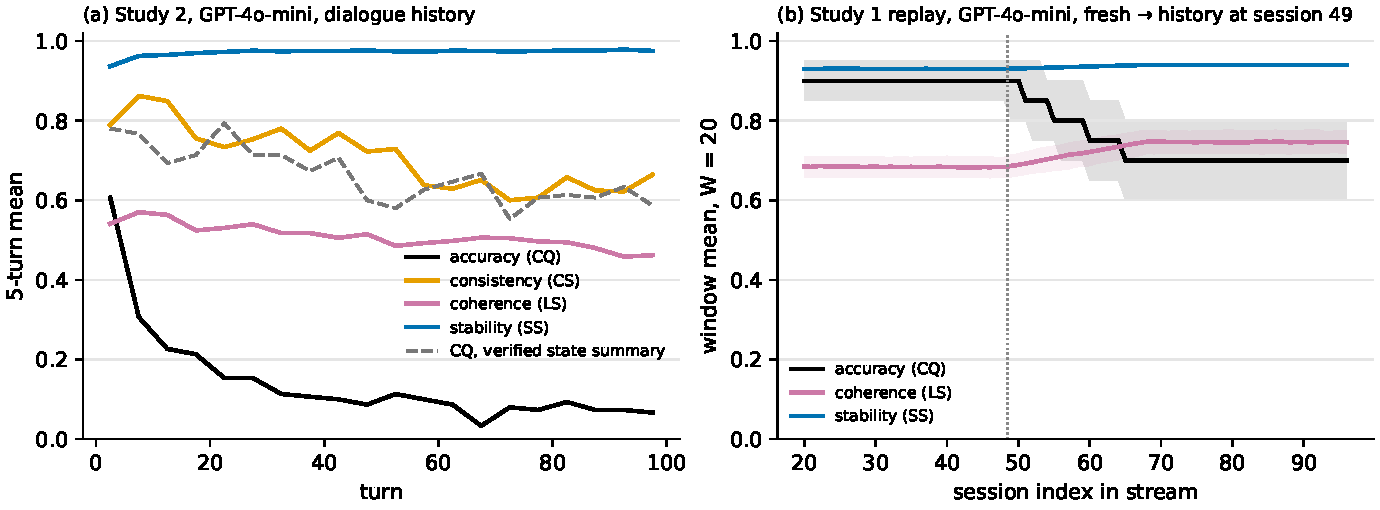
\includegraphics[width=\linewidth]{silent_metrics.pdf}
\caption{Quality metrics do not track accuracy. (a) Study 2, GPT-4o-mini,
dialogue history, 5-turn means over 30 dialogues (descriptive); dashed:
accuracy under the verified state summary; CS is supported by
\silentCsSupport{} of 3,000 turns. (b) Post-hoc replay of Study 1: median and
10--90\% band over 1,000 orderings of window means ($W=20$) when the regime
switches from fresh prefix to dialogue history at session 49.}
\label{fig:silent}
\end{figure}

\subsection{Calibrated single-stream detectors}

In the Study~1 replay (post hoc), with thresholds calibrated on 2,000
permutation nulls at family-wise $\alpha=0.05$ and validated on 2,000 disjoint
nulls, the best detection rate of any configuration was 0.067 (Mistral-7B, CQ,
sudden switch, median delay about 44 sessions); no metric qualified
(supplementary Table~S3). In this replay the stream items
are completed sessions, not turns, and a detection is any first alarm after
the switch, so the 33-turn window of Definition~2 does not apply; the delay is
counted in sessions.

In the Study~2 dialogue arm (confirmatory), the stationary dialogues that should
serve as nulls collapsed themselves. For CQ no grid value met the 5\% null
false-alarm target in most configurations, and the other metrics detected at
most 0.11 of drifts within 33 turns (supplementary
Table~S9). This is the core difficulty of monitoring under
accumulated history: the decline starts at turn~1, before any reference period,
in exactly the streams that define normal behaviour.

The verified-state arm removes this background collapse and leaves only the
scheduled task drift, so it is the cleanest test of the detectors. On
GPT-4o-mini (exploratory), CUSUM on the window mean of CQ detected
\ctrlScreenDetect{} drift dialogues within 33 turns at $W=20$, partly because
the detectors ignore their first 20 window values, which places the earliest
alarm near turn 40, after the first change at 34. A simpler rule, a window mean
below $\mu_0-2\sigma_0/\sqrt{W}$ for three turns with $\mu_0,\sigma_0$ from turns
1--30, flagged accuracy in \earlyCqSignal{} drift but also \earlyCqNull{}
stationary dialogues. LS signalled in \earlyLsSignal{} drift dialogues,
\earlyLsBefore{} of them before accuracy, but also in \earlyLsNull{} stationary
ones. Applied unchanged to the unseen Llama-3 70B and Gemma 3 12B control arms
as a frozen validation, CUSUM detected \valLlamaDetect{} and \valGemmaDetect{}
drift dialogues (median delays \valLlamaDelay{} and \valGemmaDelay{} turns),
and the LS rule signalled in \valLlamaLsSignal{} and \valGemmaLsSignal{} drift
dialogues but also in \valLlamaLsNull{} and \valGemmaLsNull{} stationary ones.
Neither rule passed the frozen screen in either model.

Because the frozen monitor cannot alarm before turn 40, part of this failure
could reflect the monitor rather than the signals. A post-hoc audit
(supplementary Section~S6) removed the floor with a CUSUM on raw values
standardised against turns 1--30. On synthetic streams it caught a precursor
injected at turn 31 by turn 33 in 45\% of streams for a shift of 0.3 and in
nearly all for 0.5, where the frozen path caught none. On the control arms,
with thresholds set on GPT-4o-mini and transferred unchanged, the CQ detector
alarmed in 0.25 and 0.17 of the stationary Llama and Gemma dialogues, and LS
or ES alarmed before CQ in at most 3 of 5 dialogues in which both alarmed
(supplementary Table~S19). No non-CQ signal combined an early alarm, a
controlled false-alarm rate and transfer across models, so the negative result
does not rest on the turn-40 floor.

\subsection{Why single streams are underpowered}

These failures follow from the information in one 100-turn stream. A simple
bound shows the scale of the problem. Consider the accuracy window mean
(\ref{eq:windowmean}) pooled over $m$ dialogues that are at the same turn, so
that it averages $n=mW$ binary outcomes.

\begin{proposition}[Smallest detectable drop]
\label{prop:mindrop}
Let the $n=mW$ outcomes in the window be independent Bernoulli variables with
success probability $p_0$ before a change and $p_1=p_0-\delta$ after it, and
write $\sigma_i^2=p_i(1-p_i)$. Consider a one-sided test that alarms when the
window mean falls below a threshold set so that its false-alarm probability
under $p_0$ is $\alpha$. Under the normal approximation, the test detects the
drop with probability at least $\beta$ only if
\begin{equation}
  \delta \;\ge\; \frac{z_{1-\alpha}\,\sigma_0 + z_{\beta}\,\sigma_1}{\sqrt{mW}},
  \label{eq:mindrop}
\end{equation}
where $z_q$ is the $q$-quantile of the standard normal distribution.
\end{proposition}

\begin{pf}
Under $p_i$ the window mean is approximately normal with mean $p_i$ and
standard deviation $\sigma_i/\sqrt{n}$. A false-alarm probability $\alpha$
requires the threshold $k=p_0-z_{1-\alpha}\sigma_0/\sqrt{n}$. Under $p_1$ the
detection probability is $\Phi\!\left((k-p_1)\sqrt{n}/\sigma_1\right)$, which is
at least $\beta$ exactly when $(k-p_1)\sqrt{n}\ge z_\beta\sigma_1$. Substituting
$k$ and $p_0-p_1=\delta$ gives (\ref{eq:mindrop}).
\end{pf}

With $p_0=0.8$, $W=20$, $\alpha=0.05$ and $\beta=0.8$, the bound is about 0.24
for one dialogue, 0.10 for six and 0.05 for 18. A monitor looks at many turns,
so its per-look level must be smaller: splitting $\alpha$ over the 67 looks
from turn 34 to turn 100 raises the bound to 0.38, 0.15 and 0.09. Positive
dependence between successive turns lowers the effective $n$ and raises it
further. The proposition covers only a threshold on the window mean, not
CUSUM or the other detectors, so it explains the scale and the $1/\sqrt{m}$
gain from aggregation rather than predicting their exact power.

To measure the power of the detectors actually used, we simulated per-turn correctness streams with pre-change accuracy 0.80 and a drop
$\delta$ at turn 34 or 51, aggregating $m$ independent dialogues per turn, with
the unchanged detectors, thresholds from 12 null streams at a 5\% false-alarm
target, and 300 drift streams per cell (Figure~\ref{fig:power}). A single
stream reached 80\% detection within 33 turns only for drops of about 0.5,
whereas the task drifts in our data were 0.1--0.3. Aggregating six dialogues
per turn lowered the detectable drop to 0.2, and 18 dialogues to 0.1; results
were similar for other windows and calibration sets (supplementary
Table~S14). Applied exploratorily to the control arms, a
CQ CUSUM on six-dialogue scenario aggregates detected all three drift
scenarios in both validation models (\valLlamaAggDetect{} and
\valGemmaAggDetect{}), with no alarm in the Llama stationary aggregates and one
in the two Gemma ones (\valLlamaAggNull{}, \valGemmaAggNull{}). Aggregation
across sessions is thus promising, but too few aggregates and the Gemma false
alarm preclude a confirmatory claim. Small null sets also limit what a clean
result can show. With no alarm in $n$ null streams, the exact one-sided 95\%
upper bound on the false-alarm rate is $1-0.05^{1/n}$: 0.78 for two aggregates
and 0.22 for 12 dialogues. Our thresholds therefore meet a 5\% target on the
calibration nulls, but the true false-alarm rate is verified only within these
bounds.

\begin{figure}[!htbp]
\centering
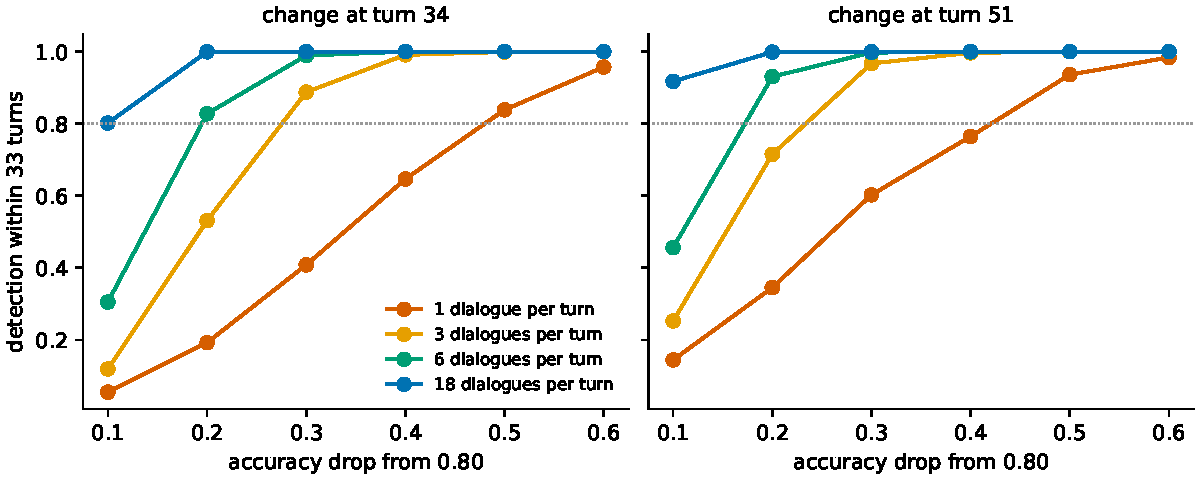
\includegraphics[width=\linewidth]{detector_power.pdf}
\caption{Simulated detection within 33 turns versus the accuracy drop from 0.80
and the number of dialogues aggregated per turn ($W=20$, thresholds from 12
null streams, 5\% false-alarm target). Left: change at turn 34; right: at
turn 51. Dotted line: 80\% detection.}
\label{fig:power}
\end{figure}

\subsection{A baseline that could not fire}

Our generic ADWIN baseline never alarmed, because our implementation omitted
the variance term of the cut bound of \citet{bifet2007learning}; without it, no
difference of means in at most 100 values in $[0,1]$ can exceed the bound.
Re-running every affected analysis with a corrected ADWIN and with CUSUM, as a
labelled sensitivity analysis, changed no conclusion: the corrected analyses
also produced no early-warning candidate for consistency or stability. Even
corrected ADWIN
needed drops of about 0.6 on 100-turn streams (supplementary
Table~S15). A generic baseline is a meaningful comparator only
once it has been shown to fire on streams of the intended length.

\section{Discussion}
\label{sec:discussion}

\paragraph{Two complementary failure modes}
On short sharded tasks, retaining the model's own replies lowered final
success, replicating the direction of \citet{huang2026benefit} under a frozen
paired analysis. Over 100 turns of state tracking the loss was far larger:
accuracy fell to about a sixth of its initial level within twenty turns, in
every scenario and for three models of different families and sizes, and a
compact verified state removed most of it. We do not claim that the short-task
effect grows causally into the long-horizon collapse, and Study~2 cannot
separate history length, the number of state updates and error accumulation,
because the verified summary changes all three. The practical finding stands:
in stateful multi-turn use, keeping the raw transcript as the only memory has a
large and avoidable accuracy cost.

\paragraph{Why quality metrics stay silent}
Consistency, coherence and stability describe local properties of responses. A
model that has adopted a wrong state can reason coherently and repeatably from
it. In our data these metrics stayed level or rose as accuracy fell, suggesting
that accumulated context makes responses more anchored rather than more
erratic, in line with reports of self-conditioning and sycophancy
\citep{sinha2025illusion,sharma2024sycophancy}. The failure mode does not
produce the incoherence or disagreement these metrics register. Two classes of
signal remain open. The first is uncertainty. Token entropy, the signal used
by ERGO \citep{khalid2025ergo}, needs token probabilities, which our protocols
did not collect. Semantic entropy \citep{farquhar2024detecting} does not: its
discrete form clusters sampled answers by meaning and needs only the samples.
Our consistency metric is related, because it also summarises agreement among
the $K$ sampled answers, but it is a pairwise agreement rate, not an entropy,
and we did not compute semantic entropy. Both semantic and token-level entropy
therefore remain untested here. The second class is counterfactual signals,
which compare the deployed context with a history-free or state-grounded
re-query and so target the anchoring directly. CRL tracked the
current gap rather than anticipating it, and comparing answers rather than
readiness is a natural next step.

\paragraph{Implications for LLM-based information systems}
Four design rules follow. \emph{Keep state outside the transcript}: where the
state can be represented explicitly, as in ledgers, inventories, protocols and
schedules, maintain it in a verified store and send the current state with each
request. In our setting this kept accuracy 0.52--0.59 above full history and
shrank the prompt at turn 100 from tens of thousands of tokens to a few
hundred. Our solver-verified summary is an upper reference; model-written
summaries should be expected to do less well. \emph{Do not rely on
single-stream quality scores}: a dashboard of one conversation's consistency,
coherence or stability will typically remain reassuring while accuracy
collapses. \emph{Monitor by comparison or aggregation}: pooling concurrent
sessions makes realistic drops detectable, and counterfactual re-queries target
the history effect itself, at the price of delayed per-session alarms or extra
calls. \emph{Test the monitor before trusting it}: verify that each detector
can fire on streams of the intended length and that its reference period is
free of the degradation to be detected.

\paragraph{Limitations}
Both studies use arithmetic and state-tracking tasks with exact answers, which
make accuracy observable but are narrower than open-ended dialogue. All models
were accessed through one academic gateway, the two studies use different
model sets, and newer models may degrade differently. The models are not the
strongest available. This is partly a property of the design: per-model
calibration needs an informative accuracy range, and a stronger open model,
Gemma~4 31B, stayed above the hard band even at the contingency levels of the
difficulty ladder and could not be calibrated (Supplementary
Section~S2.2). Testing frontier models therefore
requires a harder ladder, not only more calls. Study~1 estimates a net
effect that includes length and position differences, and Study~2's control is
a packaged intervention, not a mechanism test. Accuracy, robustness and
efficiency were unobservable before the final turn in Study~1. Study~2's CS, RS
and SS samples are complete only for GPT-4o-mini. Monitoring analyses beyond
the frozen tests are exploratory or post-hoc, two deviations for Llama-3 70B
followed gate results and are disclosed, and one investigator performed the
task audit and calibration.

\section{Conclusion}
\label{sec:conclusion}

Keeping an LLM's own replies lowered success on short multi-turn tasks, and in
100-turn state tracking the full history collapsed accuracy within about twenty
turns at matched difficulty, while a verified state summary preserved it. The
loss was silent to the monitors we tested: no quality metric, paired readiness
measure or calibrated single-stream detector gave robust, model-general early
warning, and coherence and stability often held or rose as accuracy fell.
Systems built on LLMs should keep task state outside the transcript and monitor
across sessions or against counterfactual re-queries. Open questions include
uncertainty-based and counterfactual signals, the separate roles of history
length, state load and error accumulation, and state files that models keep
and verify themselves.


\section*{Data and code availability}
All prompts, frozen protocols, configurations, analysis code and the scripts
that generate every number, table and figure in this article are publicly
available at \url{https://github.com/senolali/reasoning-monitor-3501}. The
raw model responses and derived result files are not yet in the repository; an
archival release with a persistent DOI, containing the derived data and the
model responses that the providers' terms permit to share, will be made no
later than publication.

\section*{Acknowledgements}
This work was supported by the Scientific and Technological Research Council of
T\"urkiye (T\"UB\.{I}TAK) under the 3501 programme, project number 126E663.

\section*{Declaration of competing interest}
The author declares that he has no known competing financial interests or
personal relationships that could have appeared to influence the work reported
in this paper.

\section*{CRediT authorship contribution statement}
Ali \c{S}enol: Conceptualization, Methodology, Software, Validation, Formal
analysis, Investigation, Data curation, Visualization, Writing--original draft,
Writing--review and editing, Project administration, Funding acquisition.

\section*{Declaration of generative AI and AI-assisted technologies in the manuscript preparation process}
During the preparation of this work the author used Claude (Anthropic) in an
assistive capacity, for analysis code, figure scripts and language editing. The
author designed the studies, carried out the research and reviewed and edited
all resulting content, and takes full responsibility for the content of the
published article. The language models evaluated in Studies~1 and~2 are
objects of study, not writing aids.

\bibliographystyle{elsarticle-harv}
\bibliography{references}

\end{document}
